%=+=+=+=+=+=+=+=+=+=+=+=+=+=+=+=+=+=+=+=+=+=+=+=+=+=+=+=+=+=+=+=+=+=+=+=+=+=+=+=
% Author: Mark H. Olson
% Website: https://mholson.com
% Github: https://github.com/mholson
%
% Updated: 2022-11-05 > Version 3.14159
% - adding support for minted nord color style from pygments
% - deprecating default support for listings package
% - initial Overleaf release
% Updated: 2022-07-08 > Version 3.1415
% - porting for ease of use with overleaf.com
% - changed code printing behavior by adding default support of listings pkg
% while leaving support for custom minted pkg using codeminted documentclass
% option
% Updated: 2022-04-28 > Version 3.141
% - fixed lists by removing enumitem package
% Updated: 2022-04-13 > Version 3.14
% - added optional bibliography
% - added template file
% Updated: 2022-04-13 Version 3.1
% Created: 2015-07-31 Version 3.0
%
%=+=+=+=+=+=+=+=+=+=+=+=+=+=+=+=+=+=+=+=+=+=+=+=+=+=+=+=+=+=+=+=+=+=+=+=+=+=+=+=

%=-=-=-=-=-=-=-=-=-=-=-=-=-=-=-=-=-=-=-=-=-=-=-=-=-=-=-=-=-=-=-=-=-=-=-=-=-=-=-=
% PREAMBLE :: sthlmNordDarkDemo.tex
%=-=-=-=-=-=-=-=-=-=-=-=-=-=-=-=-=-=-=-=-=-=-=-=-=-=-=-=-=-=-=-=-=-=-=-=-=-=-=-=
%
% > > >	The following beamer class options are available
%		aspectratio=169		Change aspect ratio to 16:9	
%		bibref				Include bibliography
%		sectionpages		Show section pages
%		codeminted			use minted pkg for code printing instead of listings
%							(requires additional setup & Python installed)
%		codemintedoverleaf	use minted pkg with color style support for Overleaf
% 		font sizes 			{8, 9, 10, 11, 12, 14, 17, 20} 11 Default
%
% > > > The following sthlmnord package options are available
%		mode				= dark (default)
%							= light
%=-=-=-=-=-=-=-=-=-=-=-=-=-=-=-=-=-=-=-=-=-=-=-=-=-=-=-=-=-=-=-=-=-=-=-=-=-=-=-=

\documentclass[aspectratio=169, sectionpages, codemintedoverleaf, bibref]{beamer}
% > > > Bibliography File 
\newcommand{\bibfilename}{mhoRef.bib}
% > > > Choose Theme
\usetheme[mode=light]{sthlmnord}
%\usetheme{sthlmnord}

% > > > Generate some Lorem Ipsum placeholder text for the demo.
%\usepackage{lipsum}

% > > >	Image File Paths
% 		Here you can add one or more paths to where your images are being
%		stored.  This will allow you to include only the image file 
%		name when placing it into your document.
%\graphicspath{{path1},{path2},{path3}}
\graphicspath{{./assets/}} 
% > > >	Optional use of using subfiles to make content more modular
\usepackage{subfiles}
\usepackage{listings}
\lstset{
  language         = C++,
  basicstyle       = \ttfamily,
  keywordstyle     = \color{blue}\textbf,
  commentstyle     = \color{gray},
  stringstyle      = \color{green!70!black},
  stringstyle      = \color{red},
  columns          = fullflexible,
  numbers          = left,
  numberstyle      = \scriptsize\sffamily\color{gray},
  caption          = A hello world program in \Cpp,
  xleftmargin      = 0.16\textwidth,
  xrightmargin     = 0.16\textwidth,
  showstringspaces = false,
  float,
}

% > > > Document Information
\title{Adaptive Mesh Refinement + Curvilinear Coordinate + Dissipative Particle Dynamics CODE}
\subtitle{A Summer Program at CCSE, LBL}
\newcommand{\titleAuthor}{Created by}
\author{TTNguyen (Grad Student), AJNonaka (PhD), TBLe (PhD)}
\newcommand{\titleInstitute}{Institute}
\institute{Lawrence Berkeley National Laboratory}
\newcommand{\titleMiscI}{Course}
\newcommand{\descMiscI}{Summer Program}
\newcommand{\titleMiscII}{Format}
\newcommand{\descMiscII}{\LaTeX Beamer}
\date{\today}
\titlegraphic{nordtitlelogolight}

% > > > pdf customizations via hyperref (pkg installed by beamer)
\hypersetup{
%colorlinks=true,
% You might want to disable color links for you final draft 
% AND for colors to work properly where links are included.
colorlinks=false,
linkcolor={nordNine},
citecolor={nordNine},
urlcolor={nordNine}
}

%=-=-=-=-=-=-=-=-=-=-=-=-=-=-=-=-=-=-=-=-=-=-=-=-=-=-=-=-=-=-=-=-=-=-=-=-=-=-=-=
%
%    DOCUMENT BEGINS HERE 
%
%=-=-=-=-=-=-=-=-=-=-=-=-=-=-=-=-=-=-=-=-=-=-=-=-=-=-=-=-=-=-=-=-=-=-=-=-=-=-=-=
\begin{document}

%=-=-=-=-=-=-=-=-=-=-=-=-=-=-=-=-=-=-=-=-=-=-=-=-=-=-=-=-=-=-=-=-=-=-=-=-=-=-=-=
%   TITLE START   -=-=-=-=-=-=-=-=-=-=-=-=-=-=-=-=-=-=-=-=-=-=-=-=-=-=-=-=-=-=-=
\titlepage%
%\subfile{0-slides/tex.slide.sthmlNordCover}
%   TITLE END   --==-=-=-=-=-=-=-=-=-=-=-=-=-=-=-=-=-=-=-=-=-=-=-=-=-=-=-=-=-=-=
%=-=-=-=-=-=-=-=-=-=-=-=-=-=-=-=-=-=-=-=-=-=-=-=-=-=-=-=-=-=-=-=-=-=-=-=-=-=-=-=

%=-=-=-=-=-=-=-=-=-=-=-=-=-=-=-=-=-=-=-=-=-=-=-=-=-=-=-=-=-=-=-=-=-=-=-=-=-=-=-=
%   TABLE OF CONTENTS START   -=-=-=-=-=-=-=-=-=-=-=-=-=-=-=-=-=-=-=-=-=-=-=-=-=
\begin{frame}
	\frametitle{Table of contents}
	% > > > For longer presentations use \tableofcontents[hideallsubsections] option
	%		It is also possible to manually control the entries of the table of 
	% 		contents by sections.
	%\tableofcontents[sections={1-10}]
	%\framebreak
	%\tableofcontents[sections={11-15}]
	\tableofcontents
\end{frame}
%   TABLE OF CONTENTS END   -=-=-=-=-=-=-=-=-=-=-=-=-=-=-=-=-=-=-=-=-=-=-=-=-=-=
%=-=-=-=-=-=-=-=-=-=-=-=-=-=-=-=-=-=-=-=-=-=-=-=-=-=-=-=-=-=-=-=-=-=-=-=-=-=-=-=

%=-=-=-=-=-=-=-=-=-=-=-=-=-=-=-=-=-=-=-=-=-=-=-=-=-=-=-=-=-=-=-=-=-=-=-=-=-=-=-=
% MY SECTION: Introduction
%=-=-=-=-=-=-=-=-=-=-=-=-=-=-=-=-=-=-=-=-=-=-=-=-=-=-=-=-=-=-=-=-=-=-=-=-=-=-=-=
\section{Introduction}

\subfile{my-slides/Introduction-1}
\subfile{my-slides/Introduction-2}
\subfile{my-slides/Introduction-3}
\subfile{my-slides/Introduction-4}
\subfile{my-slides/Introduction-5}
\subfile{my-slides/Introduction-6}

%=-=-=-=-=-=-=-=-=-=-=-=-=-=-=-=-=-=-=-=-=-=-=-=-=-=-=-=-=-=-=-=-=-=-=-=-=-=-=-=
%=-=-=-=-=-=-=-=-=-=-=-=-=-=-=-=-=-=-=-=-=-=-=-=-=-=-=-=-=-=-=-=-=-=-=-=-=-=-=-=
\section{Getting Started}

\subfile{my-slides/Getting_Started-1}
\subfile{my-slides/Getting_Started-2}

%=-=-=-=-=-=-=-=-=-=-=-=-=-=-=-=-=-=-=-=-=-=-=-=-=-=-=-=-=-=-=-=-=-=-=-=-=-=-=-=
%=-=-=-=-=-=-=-=-=-=-=-=-=-=-=-=-=-=-=-=-=-=-=-=-=-=-=-=-=-=-=-=-=-=-=-=-=-=-=-=
\section{Methodologies}

\subfile{my-slides/Methodologies-1}
%   SUBSECTION    ++++++++++++++++++++++++++++++++++++++++++++++++++++++++++++++
\subsection{LM Mod to KM Scheme}

\subfile{my-slides/Methodologies-2}
\subfile{my-slides/Methodologies-3}
\subfile{my-slides/Methodologies-4}
\subfile{my-slides/Methodologies-5}
%\subfile{my-slides/Methodologies-6}

%   SUBSECTION    ++++++++++++++++++++++++++++++++++++++++++++++++++++++++++++++
\subsection{QUICK and related convection-diffusion schemes}

%   FRAME START   -=-=-=-=-=-=-=-=-=-=-=-=-=-=-=-=-=-=-=-=-=-=-=-=-=-=-=-=-=-=-=
\begin{frame}[allowframebreaks, allowdisplaybreaks, c, fragile]{Numerical Method}{2D Incompressible Fluid Dynamics}
    
    \begin{block}{}
        \begin{center}
            B. P. Leonard's Quadratic Upstream Interpolation for Convective Kinematics (QUICK).
        \end{center}
    \end{block}

    \vspace{1em}
    
    \begin{center}
        \large{The full papers can be found at:} \\
        \url{https://doi.org/10.1016/0045-7825(79)90034-3}\\
        \url{https://doi.org/10.1016/0307-904X(95)00084-W}
                
        %\begin{figure}
        %    \centerline{
\includegraphics[width=0.1\textwidth]{assets/elsevier}}
        %    \caption{Hosted on Elsevier}
        %\end{figure}
        
    \end{center}
            
\end{frame}
%   FRAME END   --==-=-=-=-=-=-=-=-=-=-=-=-=-=-=-=-=-=-=-=-=-=-=-=-=-=-=-=-=-=-=

%   FRAME START   -=-=-=-=-=-=-=-=-=-=-=-=-=-=-=-=-=-=-=-=-=-=-=-=-=-=-=-=-=-=-=
\begin{frame}[allowframebreaks, allowdisplaybreaks, t, fragile]{QUICK}{Convective terms}

    \prob Consider a non-dimensional convection-diffusion equation with constant coefficients in 1D coordinate system such that: \begin{equation}
	    \frac{\partial U}{\partial x} = \frac{1}{\mathcal{Pe}} \frac{\partial^2 U}{\partial x^2} + S(x)
 	\end{equation}

    \framebreak
    
    \soln QUICK(1/8) convection scheme with the "left-right" notation is as follow: \begin{equation}
	    \left( \frac{\partial U}{\partial x} \right)_i = \frac{U_r (i) - U_l (i)}{h}
        \label{eq:quickc}
	\end{equation}

    While $U_r$ and $U_l$ are linear interpolation of left and right wall values of $U$ such that: \begin{align}
        \left( U_r \right)^{\text{QUICK}} (i) &= \frac{1}{2} \left( U_{i+1} + U_i \right) - \frac{1}{8} \left( U_{i+1} - 2 U_i + U_{i-1} \right) \label{eq:rightwall} \\
        \left( U_l \right)^{\text{QUICK}} (i) &= \left( U_r \right)^{\text{QUICK}} (i-1) \label{eq:leftwall}
    \end{align}

    Substituting above values from Eqs.(\ref{eq:rightwall}) and (\ref{eq:leftwall}) into Eq. (\ref{eq:quickc}) gives: \begin{align}
        \left( \frac{\partial U}{\partial x} \right)_i &= \frac{1}{2} \left( U_{i+1} + U_i \right) - \frac{1}{8} \left( U_{i+1} - 2 U_i + U_{i-1} \right) - \frac{1}{2} \left( U_i + U_{i-1} \right) - \frac{1}{8} \left( U_i - 2 U_{i-1} + U_{i-2} \right) \\
        &= \frac{3 U_{i+1} + 3 U_i - 7 U_{i-1} + U_{i-2}}{8h}
    \end{align}
    
\end{frame}
%   FRAME END   --==-=-=-=-=-=-=-=-=-=-=-=-=-=-=-=-=-=-=-=-=-=-=-=-=-=-=-=-=-=-=

%   FRAME START   -=-=-=-=-=-=-=-=-=-=-=-=-=-=-=-=-=-=-=-=-=-=-=-=-=-=-=-=-=-=-=
\begin{frame}[allowframebreaks, allowdisplaybreaks, t, fragile]{Full QUICK}{Diffusive terms}
    
    QUICK technique can also be applied for the second derivative of the diffusive terms as follow: \begin{equation}
	    \frac{1}{\mathcal{Pe}} \left( \frac{\partial^2 U}{\partial x^2} \right)_i = \frac{1}{\mathcal{Pe}} \frac{U_r' (i) - U_l' (i)}{h}
        \label{eq:quickd}
	\end{equation}

    $U_r'$ is defined by taking the central difference of two neighboring nodes, such that: \begin{align}
        \left( U_r' \right)^{\text{QUICK}} (i) &= \frac{\left( U_{i+1} - U_i \right)}{h} \\
        \left( U_l' \right)^{\text{QUICK}} (i) &= \left( U_r' \right)^{\text{QUICK}} (i-1)
    \end{align}

    In similar manner, one has: \begin{equation}
        \frac{1}{\mathcal{Pe}} \left( \frac{\partial^2 U}{\partial x^2} \right)_i = \frac{1}{\mathcal{Pe}} \frac{ U_{i+1} - 2 U_i + U_{i-1} }{h^2}
    \end{equation}
    
\end{frame}
%   FRAME END   --==-=-=-=-=-=-=-=-=-=-=-=-=-=-=-=-=-=-=-=-=-=-=-=-=-=-=-=-=-=-=

%   FRAME START   -=-=-=-=-=-=-=-=-=-=-=-=-=-=-=-=-=-=-=-=-=-=-=-=-=-=-=-=-=-=-=
\begin{frame}[allowframebreaks, allowdisplaybreaks, t, fragile]{QUICK}{Summary}

    \remarks Convection-diffusion operators:

    Full QUICK: \begin{equation}
        \text{[QUICK]} = \left( \frac{3 U_{i+1} + 3 U_i - 7 U_{i-1} + U_{i-2}}{8h} \right) - \frac{1}{\mathcal{Pe}} \frac{ U_{i+1} - 2 U_i + U_{i-1} }{h^2}
    \end{equation}

    SPUDS-plus-CDS2: \begin{equation}
        \text{[SPUDS + CDS2]} = \left( \frac{2 U_{i+1} + 3 U_i - 6 U_{i-1} + U_{i-2}}{6h} \right) - \frac{1}{\mathcal{Pe}} \frac{ U_{i+1} - 2 U_i + U_{i-1} }{h^2}
    \end{equation}

    \framebreak
    
    \remarks From Leonard (1995):
    \begin{itemize}
        \item QUICK operators for the convective terms, notated by QUICK[C], are third-order accurate -- $O(h^3)$.
        \item QUICK operators for the diffusive terms, notated by QUICK[D], are only second-order accurate -- $O(h^2)$.
        \item If a finite-volume (OA) discrete operator is viewed as an finite-difference (SP) term, there is an $O(h^2)$ discrepancy between the two. A third (or higher) order OA scheme is only second-order accurate when viewed as an SP scheme, and vice versa.
    \end{itemize}
    
\end{frame}
%   FRAME END   --==-=-=-=-=-=-=-=-=-=-=-=-=-=-=-=-=-=-=-=-=-=-=-=-=-=-=-=-=-=-=

%   SUBSECTION    ++++++++++++++++++++++++++++++++++++++++++++++++++++++++++++++
\subsection{Implementation}
\subfile{my-slides/Math-1}

%   FRAME START   -=-=-=-=-=-=-=-=-=-=-=-=-=-=-=-=-=-=-=-=-=-=-=-=-=-=-=-=-=-=-=
\begin{frame}[allowframebreaks, allowdisplaybreaks, t, fragile]{Viscous Terms}{CDS2 Scheme}

	Now let us find the expression for the finite difference operators in Eq.(\ref{eq:viscous_terms}) and Eq.(\ref{eq:convective_terms}).
 
    \prob First, consider the Viscous term (\ref{eq:viscous_terms}) as follows: \begin{equation}
        L (u_i) = \frac{1}{\mathcal{Re}} \frac{\partial^2 u_i}{\partial x_j \partial x_j}
    \end{equation}

    For a 2 dimensional coordinate system, one has the expression such that:
    \\
    In x-direction: \begin{equation}
        L_x (u) = \frac{1}{\mathcal{Re}} \left( \frac{\partial^2 u}{\partial x^2} + \frac{\partial^2 u}{\partial y^2} \right)
    \end{equation}

    In y-direction: \begin{equation}
        L_y (v) = \frac{1}{\mathcal{Re}} \left( \frac{\partial^2 v}{\partial x^2} + \frac{\partial^2 v}{\partial y^2} \right)
    \end{equation}

    \framebreak

    The second derivative at an arbitrary point $(i, j)$ is approximated by the second central difference: \begin{align}
        \frac{\partial^2 u_{i,j}}{\partial x^2} &= \frac{u_{i+1,j} - 2 u_{i,j} + u_{i-1,j}}{\Delta x^2} \\
        \frac{\partial^2 u_{i,j}}{\partial y^2} &= \frac{u_{i,j+1} - 2 u_{i,j} + u_{i,j-1}}{\Delta y^2}
    \end{align}

    and: \begin{align}
        \frac{\partial^2 v_{i,j}}{\partial x^2} &= \frac{v_{i+1,j} - 2 v_{i,j} + v_{i-1,j}}{\Delta x^2} \\
        \frac{\partial^2 v_{i,j}}{\partial y^2} &= \frac{v_{i,j+1} - 2 v_{i,j} + v_{i,j-1}}{\Delta y^2}
    \end{align}
        
\end{frame}
%   FRAME END   --==-=-=-=-=-=-=-=-=-=-=-=-=-=-=-=-=-=-=-=-=-=-=-=-=-=-=-=-=-=-=

%   FRAME START   -=-=-=-=-=-=-=-=-=-=-=-=-=-=-=-=-=-=-=-=-=-=-=-=-=-=-=-=-=-=-=
\begin{frame}[c]{Viscous Flux Calculation in Code}
    \begin{center}
        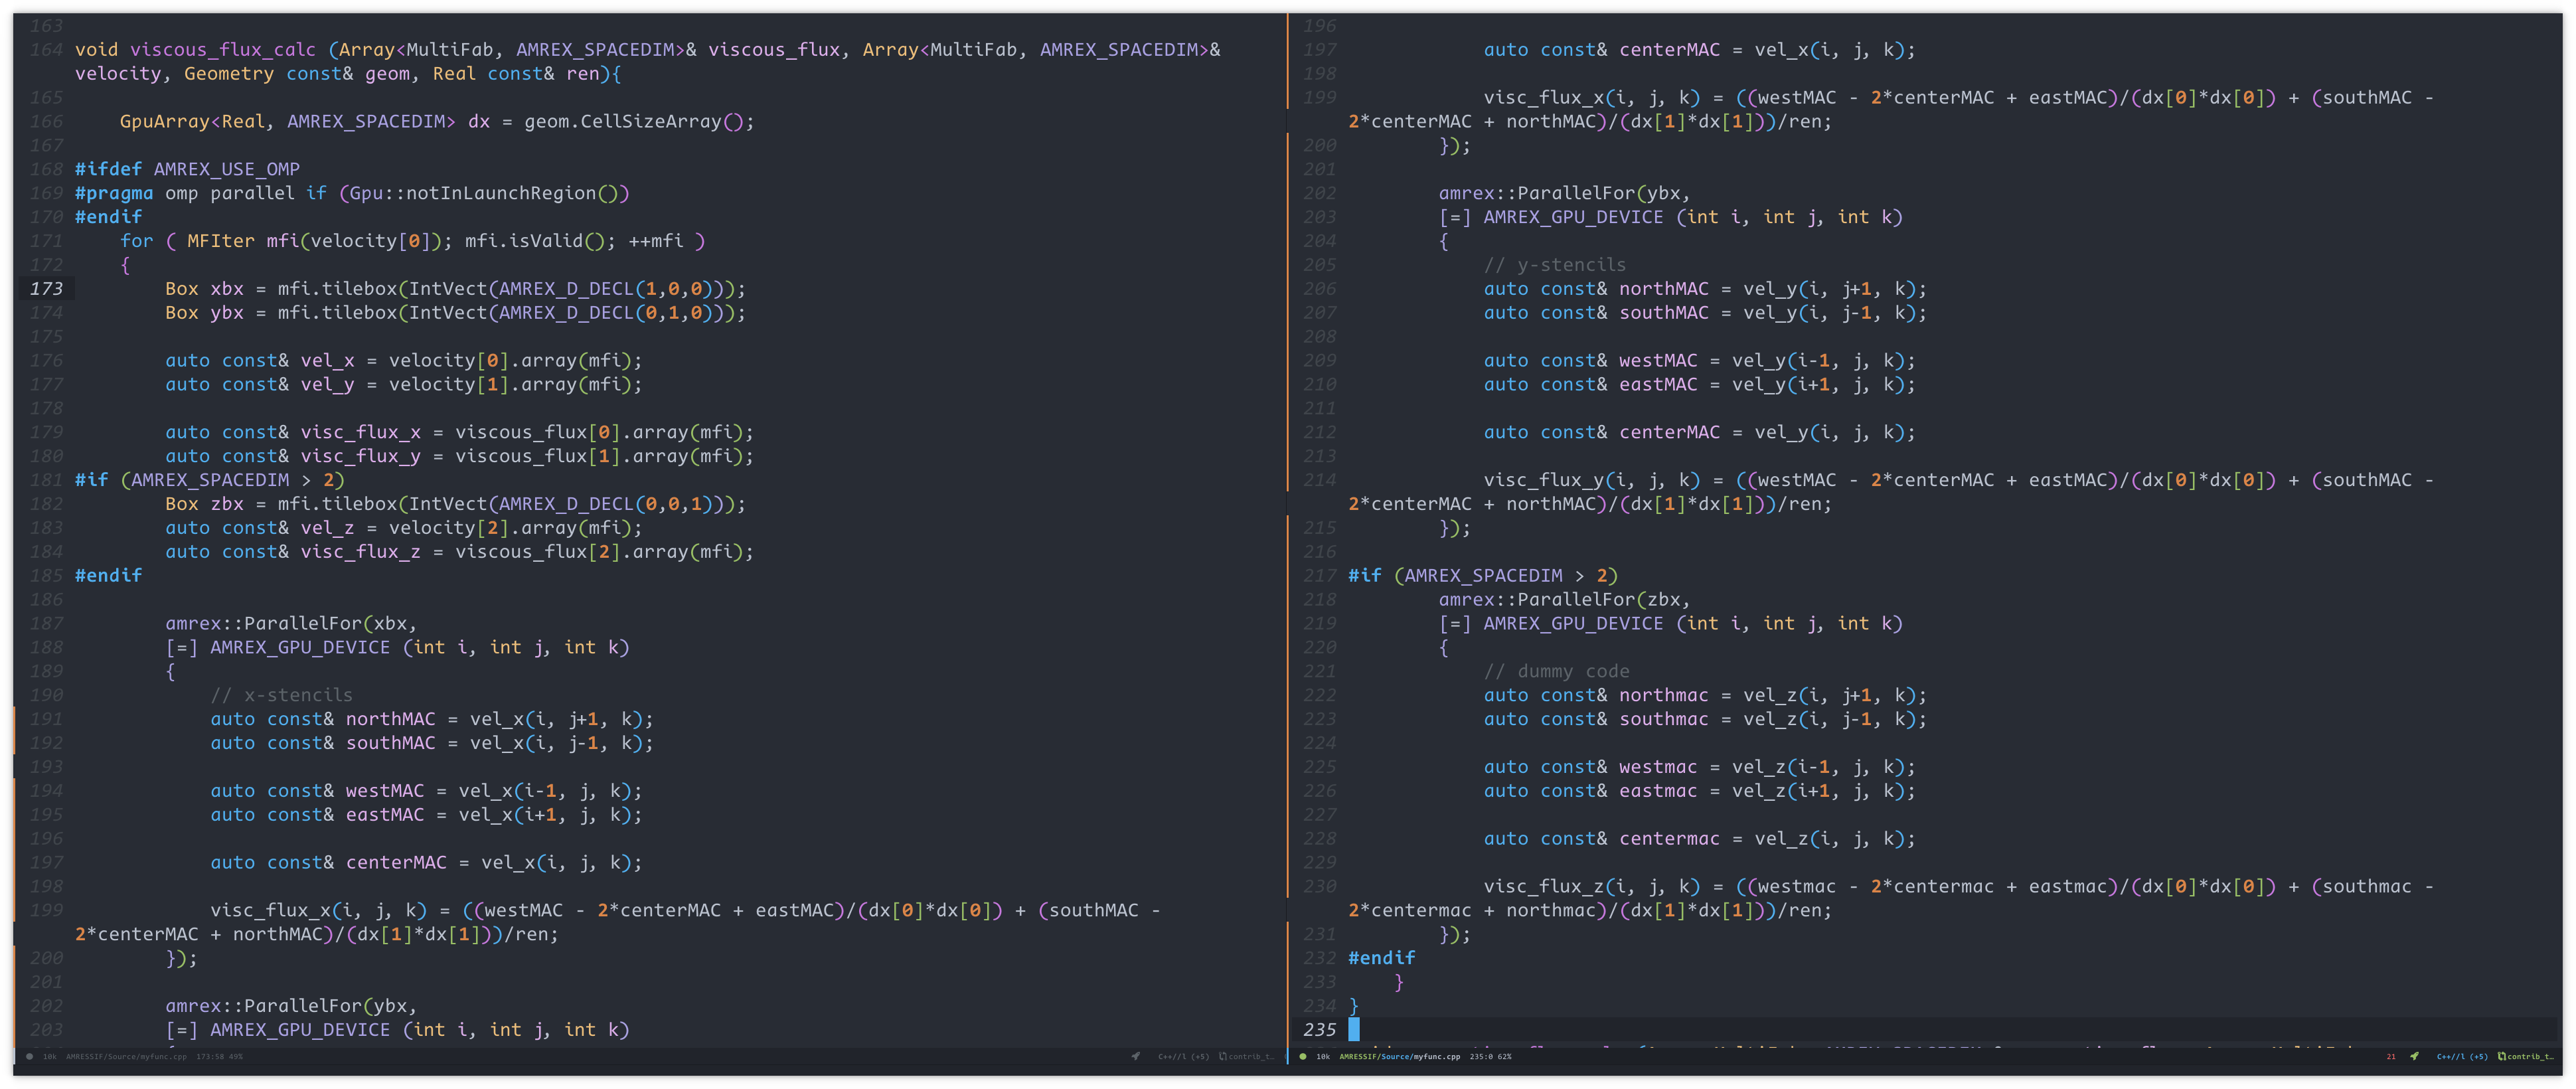
\includegraphics[width=\textwidth]{viscous_term}
    \end{center}
\end{frame}
%   FRAME END   -=-=-=-=-=-=-=-=-=-=-=-=-=-=-=-=-=-=-=-=-=-=-=-=-=-=-=-=-=-=-=

%   FRAME START   -=-=-=-=-=-=-=-=-=-=-=-=-=-=-=-=-=-=-=-=-=-=-=-=-=-=-=-=-=-=-=
\begin{frame}[allowframebreaks, allowdisplaybreaks, t, fragile]{Convective Terms}{QUICK Scheme}

	Now let us find the expression for the finite difference operators in Eq.(\ref{eq:viscous_terms}) and Eq.(\ref{eq:convective_terms}).
 
    \prob First, consider the Viscous term (\ref{eq:viscous_terms}) as follows: \begin{equation}
        L (u_i) = \frac{1}{\mathcal{Re}} \frac{\partial^2 u_i}{\partial x_j \partial x_j}
    \end{equation}

    For a 2 dimensional coordinate system, one has the expression such that:
    \\
    In x-direction: \begin{equation}
        L_x (u) = \frac{1}{\mathcal{Re}} \left( \frac{\partial^2 u}{\partial x^2} + \frac{\partial^2 u}{\partial y^2} \right)
    \end{equation}

    In y-direction: \begin{equation}
        L_y (v) = \frac{1}{\mathcal{Re}} \left( \frac{\partial^2 v}{\partial x^2} + \frac{\partial^2 v}{\partial y^2} \right)
    \end{equation}

    \framebreak

    The second derivative at an arbitrary point $(i, j)$ is approximated by the second central difference: \begin{align}
        \frac{\partial^2 u_{i,j}}{\partial x^2} &= \frac{u_{i+1,j} - 2 u_{i,j} + u_{i-1,j}}{\Delta x^2} \\
        \frac{\partial^2 u_{i,j}}{\partial y^2} &= \frac{u_{i,j+1} - 2 u_{i,j} + u_{i,j-1}}{\Delta y^2}
    \end{align}

    and: \begin{align}
        %\frac{\partial^2 v_{i,j}}{\partial x^2} &= \frac{v_{i+1,j} - 2 v_{i,j} + v_{i-1,j}}{\Delta x^2} \\
        %\frac{\partial^2 v_{i,j}}{\partial y^2} &= \frac{v_{i,j+1} - 2 v_{i,j} + v_{i,j-1}}{\Delta y^2}
        u(x,y)^{t=0} &= - \cos{(2 \pi x)}*\sin{(2 \pi y)} \\
        v(x,y)^{t=0} &= \sin{(2 \pi x)}*\cos{(2 \pi y)}
    \end{align}
        
\end{frame}
%   FRAME END   --==-=-=-=-=-=-=-=-=-=-=-=-=-=-=-=-=-=-=-=-=-=-=-=-=-=-=-=-=-=-=

%   FRAME START   -=-=-=-=-=-=-=-=-=-=-=-=-=-=-=-=-=-=-=-=-=-=-=-=-=-=-=-=-=-=-=
\begin{frame}[allowframebreaks, allowdisplaybreaks, t, fragile]{Implementation}{JASSIF.jl}

	For inner nodes:
    \begin{equation}
        \begin{split}
            F &= um \left[ 1/8 * \left( -U_{i+2} - 2 U_{i+1} + 3 U_{i} \right) + U_{i+1} \right] \\
            &+ up \left[ 1/8 * \left( -U_{i-1} - 2 U_{i} + 3 U_{i+1} \right) + U_{i} \right]
        \end{split}
	\end{equation}

    For begin node ($i=1$):
    \begin{equation}
        \begin{split}
            F &= um \left[ 1/8 * \left( -U_{i+2} - 2 U_{i+1} + 3 U_{i} \right) + U_{i+1} \right] \\
            &+ up \left[ 1/8 * \left( -U_{i} - 2 U_{i} + 3 U_{i+1} \right) + U_{i} \right]
        \end{split}
	\end{equation}

    For end node ($i=N$):
    \begin{equation}
        \begin{split}
            F &= um \left[ 1/8 * \left( -U_{i+1} - 2 U_{i+1} + 3 U_{i} \right) + U_{i+1} \right] \\
            &+ up \left[ 1/8 * \left( -U_{i-1} - 2 U_{i} + 3 U_{i+1} \right) + U_{i} \right]
        \end{split}
	\end{equation}
        
\end{frame}
%   FRAME END   --==-=-=-=-=-=-=-=-=-=-=-=-=-=-=-=-=-=-=-=-=-=-=-=-=-=-=-=-=-=-=

%   SUBSECTION    ++++++++++++++++++++++++++++++++++++++++++++++++++++++++++++++
\subsection{Preconditioned Jacobian-free Newton-Krylov}
%   FRAME START   -=-=-=-=-=-=-=-=-=-=-=-=-=-=-=-=-=-=-=-=-=-=-=-=-=-=-=-=-=-=-=
\begin{frame}[c]{JFNK}
    \begin{center}
        \Large{What is that?}
    \end{center}
\end{frame}
%   FRAME END   -=-=-=-=-=-=-=-=-=-=-=-=-=-=-=-=-=-=-=-=-=-=-=-=-=-=-=-=-=-=-=

%   SUBSECTION    ++++++++++++++++++++++++++++++++++++++++++++++++++++++++++++++
\subsection{Julian Solver for Incompressible Flow}
%   FRAME START   -=-=-=-=-=-=-=-=-=-=-=-=-=-=-=-=-=-=-=-=-=-=-=-=-=-=-=-=-=-=-=
\begin{frame}[allowframebreaks, allowdisplaybreaks, t, fragile]{Julian Solver}{Overview}

	\begin{center}
        \large{Code structure:}
        \\
        \vspace{1em}
        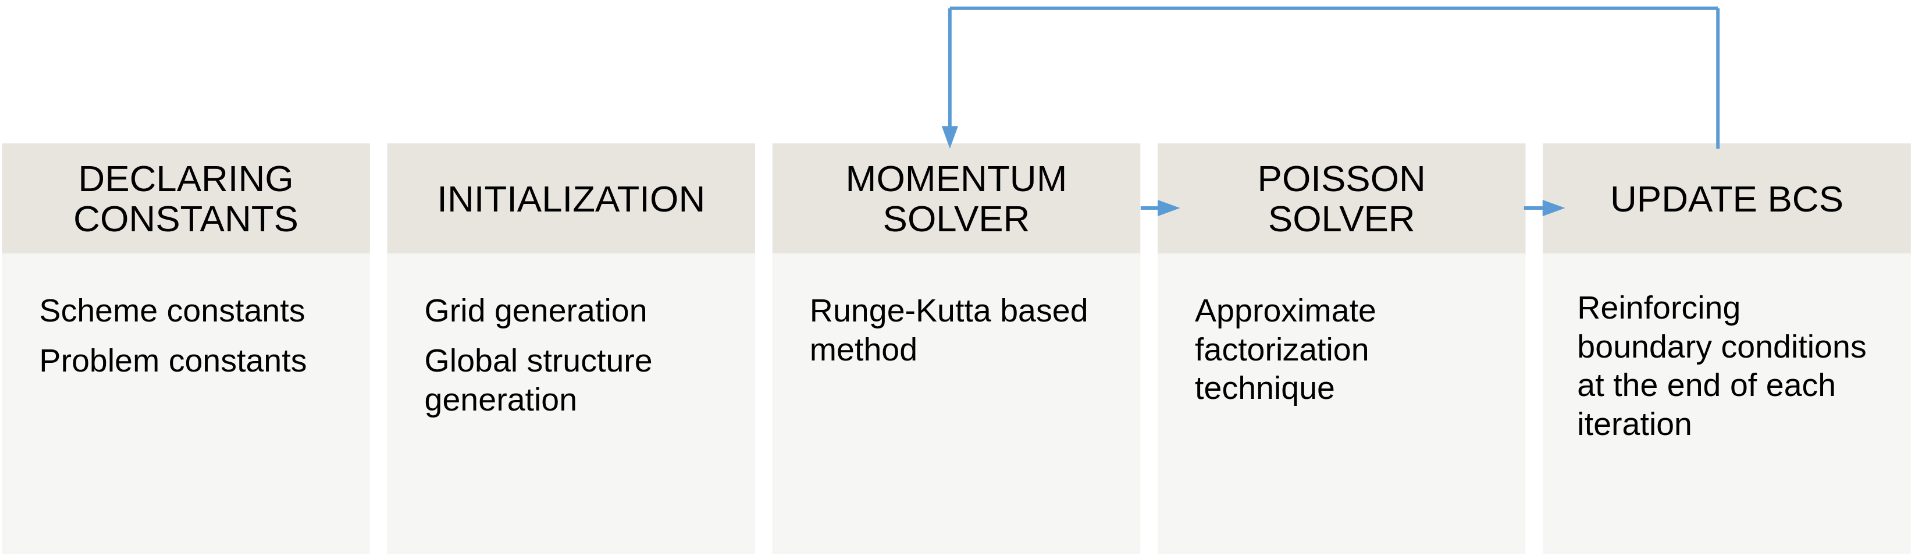
\includegraphics[width=0.9\textwidth]{julia}
    \end{center}

\end{frame}
%   FRAME END   --==-=-=-=-=-=-=-=-=-=-=-=-=-=-=-=-=-=-=-=-=-=-=-=-=-=-=-=-=-=-=

\subfile{my-slides/Julia-Main}
\subfile{my-slides/Julia-Momentum}
\subfile{my-slides/Julia-Poisson}
\subfile{my-slides/Julia-Update}
\subfile{my-slides/Julia-Boundary_Conditions}

%=-=-=-=-=-=-=-=-=-=-=-=-=-=-=-=-=-=-=-=-=-=-=-=-=-=-=-=-=-=-=-=-=-=-=-=-=-=-=-=
%=-=-=-=-=-=-=-=-=-=-=-=-=-=-=-=-=-=-=-=-=-=-=-=-=-=-=-=-=-=-=-=-=-=-=-=-=-=-=-=
\section{Results}

\subfile{my-slides/Results-1}
\subfile{my-slides/Results-2}
\subfile{my-slides/Results-3}

%=-=-=-=-=-=-=-=-=-=-=-=-=-=-=-=-=-=-=-=-=-=-=-=-=-=-=-=-=-=-=-=-=-=-=-=-=-=-=-=

%=-=-=-=-=-=-=-=-=-=-=-=-=-=-=-=-=-=-=-=-=-=-=-=-=-=-=-=-=-=-=-=-=-=-=-=-=-=-=-=
%=-=-=-=-=-=-=-=-=-=-=-=-=-=-=-=-=-=-=-=-=-=-=-=-=-=-=-=-=-=-=-=-=-=-=-=-=-=-=-=
\section{Meeting Minutues}

\subfile{my-slides/Meeting_Minutes-1}

%=-=-=-=-=-=-=-=-=-=-=-=-=-=-=-=-=-=-=-=-=-=-=-=-=-=-=-=-=-=-=-=-=-=-=-=-=-=-=-=

%=-=-=-=-=-=-=-=-=-=-=-=-=-=-=-=-=-=-=-=-=-=-=-=-=-=-=-=-=-=-=-=-=-=-=-=-=-=-=-=
% DEFAULT SECTIONS 
%=-=-=-=-=-=-=-=-=-=-=-=-=-=-=-=-=-=-=-=-=-=-=-=-=-=-=-=-=-=-=-=-=-=-=-=-=-=-=-=
%\section{Background Information}

%\subfile{0-slides/tex.slide.useMetroWarning}
%\subfile{0-slides/tex.slide.majorFeatures}
%\subfile{0-slides/tex.slide.history}
%\subfile{0-slides/tex.slide.noGuarantee}
%\subfile{0-slides/tex.slide.availableGitHub}
%\subfile{0-slides/tex.slide.availableOverleaf}
%\subfile{0-slides/tex.slide.ctanPackages}
%\subfile{0-slides/tex.slide.customPackages}

%=-=-=-=-=-=-=-=-=-=-=-=-=-=-=-=-=-=-=-=-=-=-=-=-=-=-=-=-=-=-=-=-=-=-=-=-=-=-=-=
%=-=-=-=-=-=-=-=-=-=-=-=-=-=-=-=-=-=-=-=-=-=-=-=-=-=-=-=-=-=-=-=-=-=-=-=-=-=-=-=
%\section{Colors}

%\subfile{0-slides/tex.slide.nordPaletteDark}
\subfile{0-slides/tex.slide.nordPaletteTextDark}
%\subfile{0-slides/tex.slide.nordPaletteTextHighlightDark}

%=-=-=-=-=-=-=-=-=-=-=-=-=-=-=-=-=-=-=-=-=-=-=-=-=-=-=-=-=-=-=-=-=-=-=-=-=-=-=-=
%=-=-=-=-=-=-=-=-=-=-=-=-=-=-=-=-=-=-=-=-=-=-=-=-=-=-=-=-=-=-=-=-=-=-=-=-=-=-=-=
%\section{Deck Structures}

%\subfile{0-slides/tex.slide.blocks}
%\subfile{0-slides/tex.slide.listsEnumerate}
%\subfile{0-slides/tex.slide.listsItemize}
%\subfile{0-slides/tex.slide.listsDescription}
%\subfile{0-slides/tex.slide.codeblocks}

%\subfile{0-slides/tex.slide.exampleSlide}
%\subfile{0-slides/tex.slide.theoremSlide}

%=-=-=-=-=-=-=-=-=-=-=-=-=-=-=-=-=-=-=-=-=-=-=-=-=-=-=-=-=-=-=-=-=-=-=-=-=-=-=-=
%=-=-=-=-=-=-=-=-=-=-=-=-=-=-=-=-=-=-=-=-=-=-=-=-=-=-=-=-=-=-=-=-=-=-=-=-=-=-=-=
%\section{Fonts}

%\subfile{0-slides/tex.slide.fonts}

%=-=-=-=-=-=-=-=-=-=-=-=-=-=-=-=-=-=-=-=-=-=-=-=-=-=-=-=-=-=-=-=-=-=-=-=-=-=-=-=
%=-=-=-=-=-=-=-=-=-=-=-=-=-=-=-=-=-=-=-=-=-=-=-=-=-=-=-=-=-=-=-=-=-=-=-=-=-=-=-=
%\section{Mathematics}

%\subfile{0-slides/tex.slide.typeMathematics}
%\subfile{0-slides/tex.slide.tikz}
%\subfile{0-slides/tex.slide.mathExampleExpand}

%\subfile{0-slides/tex.slide.mathExampleCTS}
%\subfile{0-slides/tex.slide.mathExampleDiceCoins.tex}
%\subfile{0-slides/tex.slide.mathSets}

%=-=-=-=-=-=-=-=-=-=-=-=-=-=-=-=-=-=-=-=-=-=-=-=-=-=-=-=-=-=-=-=-=-=-=-=-=-=-=-=
%=-=-=-=-=-=-=-=-=-=-=-=-=-=-=-=-=-=-=-=-=-=-=-=-=-=-=-=-=-=-=-=-=-=-=-=-=-=-=-=
\section{References}

\begin{frame}[allowframebreaks]{References}
    \printbibliography[title={References}]%
\end{frame}

%=-=-=-=-=-=-=-=-=-=-=-=-=-=-=-=-=-=-=-=-=-=-=-=-=-=-=-=-=-=-=-=-=-=-=-=-=-=-=-=
\end{document}
%=+=+=+=+=+=+=+=+=+=+=+=+=+=+=+=+=+=+=+=+=+=+=+=+=+=+=+=+=+=+=+=+=+=+=+=+=+=+=+=
% END OF FILE
%=+=+=+=+=+=+=+=+=+=+=+=+=+=+=+=+=+=+=+=+=+=+=+=+=+=+=+=+=+=+=+=+=+=+=+=+=+=+=+=